% Options for packages loaded elsewhere
% Options for packages loaded elsewhere
\PassOptionsToPackage{unicode}{hyperref}
\PassOptionsToPackage{hyphens}{url}
\PassOptionsToPackage{dvipsnames,svgnames,x11names}{xcolor}
%
\documentclass[
  indonesian,
]{agujournal2019}
\usepackage{xcolor}
\usepackage{amsmath,amssymb}
\setcounter{secnumdepth}{5}
\usepackage{iftex}
\ifPDFTeX
  \usepackage[T1]{fontenc}
  \usepackage[utf8]{inputenc}
  \usepackage{textcomp} % provide euro and other symbols
\else % if luatex or xetex
  \usepackage{unicode-math} % this also loads fontspec
  \defaultfontfeatures{Scale=MatchLowercase}
  \defaultfontfeatures[\rmfamily]{Ligatures=TeX,Scale=1}
\fi
\usepackage{lmodern}
\ifPDFTeX\else
  % xetex/luatex font selection
\fi
% Use upquote if available, for straight quotes in verbatim environments
\IfFileExists{upquote.sty}{\usepackage{upquote}}{}
\IfFileExists{microtype.sty}{% use microtype if available
  \usepackage[]{microtype}
  \UseMicrotypeSet[protrusion]{basicmath} % disable protrusion for tt fonts
}{}
\makeatletter
\@ifundefined{KOMAClassName}{% if non-KOMA class
  \IfFileExists{parskip.sty}{%
    \usepackage{parskip}
  }{% else
    \setlength{\parindent}{0pt}
    \setlength{\parskip}{6pt plus 2pt minus 1pt}}
}{% if KOMA class
  \KOMAoptions{parskip=half}}
\makeatother
% Make \paragraph and \subparagraph free-standing
\makeatletter
\ifx\paragraph\undefined\else
  \let\oldparagraph\paragraph
  \renewcommand{\paragraph}{
    \@ifstar
      \xxxParagraphStar
      \xxxParagraphNoStar
  }
  \newcommand{\xxxParagraphStar}[1]{\oldparagraph*{#1}\mbox{}}
  \newcommand{\xxxParagraphNoStar}[1]{\oldparagraph{#1}\mbox{}}
\fi
\ifx\subparagraph\undefined\else
  \let\oldsubparagraph\subparagraph
  \renewcommand{\subparagraph}{
    \@ifstar
      \xxxSubParagraphStar
      \xxxSubParagraphNoStar
  }
  \newcommand{\xxxSubParagraphStar}[1]{\oldsubparagraph*{#1}\mbox{}}
  \newcommand{\xxxSubParagraphNoStar}[1]{\oldsubparagraph{#1}\mbox{}}
\fi
\makeatother


\usepackage{longtable,booktabs,array}
\newcounter{none} % for unnumbered tables
\usepackage{calc} % for calculating minipage widths
% Correct order of tables after \paragraph or \subparagraph
\usepackage{etoolbox}
\makeatletter
\patchcmd\longtable{\par}{\if@noskipsec\mbox{}\fi\par}{}{}
\makeatother
% Allow footnotes in longtable head/foot
\IfFileExists{footnotehyper.sty}{\usepackage{footnotehyper}}{\usepackage{footnote}}
\makesavenoteenv{longtable}
\usepackage{graphicx}
\makeatletter
\newsavebox\pandoc@box
\newcommand*\pandocbounded[1]{% scales image to fit in text height/width
  \sbox\pandoc@box{#1}%
  \Gscale@div\@tempa{\textheight}{\dimexpr\ht\pandoc@box+\dp\pandoc@box\relax}%
  \Gscale@div\@tempb{\linewidth}{\wd\pandoc@box}%
  \ifdim\@tempb\p@<\@tempa\p@\let\@tempa\@tempb\fi% select the smaller of both
  \ifdim\@tempa\p@<\p@\scalebox{\@tempa}{\usebox\pandoc@box}%
  \else\usebox{\pandoc@box}%
  \fi%
}
% Set default figure placement to htbp
\def\fps@figure{htbp}
\makeatother



\ifLuaTeX
\usepackage[bidi=basic,shorthands=off,provide=*]{babel}
\else
\usepackage[bidi=default,shorthands=off,provide=*]{babel}
\fi
\ifLuaTeX
  \usepackage{selnolig} % disable illegal ligatures
\fi


\setlength{\emergencystretch}{3em} % prevent overfull lines

\providecommand{\tightlist}{%
  \setlength{\itemsep}{0pt}\setlength{\parskip}{0pt}}



 


\usepackage{booktabs}
\usepackage{caption}
\usepackage{longtable}
\usepackage{colortbl}
\usepackage{array}
\usepackage{anyfontsize}
\usepackage{multirow}
\usepackage{url} %this package should fix any errors with URLs in refs.
\usepackage{lineno}
\usepackage[inline]{trackchanges} %for better track changes. finalnew option will compile document with changes incorporated.
\usepackage{soul}
\linenumbers
\makeatletter
\@ifpackageloaded{caption}{}{\usepackage{caption}}
\AtBeginDocument{%
\ifdefined\contentsname
  \renewcommand*\contentsname{Daftar Isi}
\else
  \newcommand\contentsname{Daftar Isi}
\fi
\ifdefined\listfigurename
  \renewcommand*\listfigurename{Daftar Gambar}
\else
  \newcommand\listfigurename{Daftar Gambar}
\fi
\ifdefined\listtablename
  \renewcommand*\listtablename{Daftar Tabel}
\else
  \newcommand\listtablename{Daftar Tabel}
\fi
\ifdefined\figurename
  \renewcommand*\figurename{Gambar}
\else
  \newcommand\figurename{Gambar}
\fi
\ifdefined\tablename
  \renewcommand*\tablename{Tabel}
\else
  \newcommand\tablename{Tabel}
\fi
}
\@ifpackageloaded{float}{}{\usepackage{float}}
\floatstyle{ruled}
\@ifundefined{c@chapter}{\newfloat{codelisting}{h}{lop}}{\newfloat{codelisting}{h}{lop}[chapter]}
\floatname{codelisting}{Daftar}
\newcommand*\listoflistings{\listof{codelisting}{Daftar Daftar}}
\captionsetup{labelsep=period}
\makeatother
\makeatletter
\makeatother
\makeatletter
\@ifpackageloaded{caption}{}{\usepackage{caption}}
\@ifpackageloaded{subcaption}{}{\usepackage{subcaption}}
\makeatother
\usepackage{bookmark}
\IfFileExists{xurl.sty}{\usepackage{xurl}}{} % add URL line breaks if available
\urlstyle{same}
\hypersetup{
  pdftitle={Kombinasi TyHbA1c Index{,} Usia{,} dan Indeks Massa Tubuh sebagai Prediktor High-Risk Plaque pada Pasien Diabetes Mellitus: Sebuah Pendekatan Nomogram Klinis},
  pdfauthor={Kadek Adit Wiryadana},
  pdflang={id},
  pdfkeywords={Indeks TyHbA1c, High-Risk Plaque, Computed Tomography
Coronary Angiography, Nomogram Klinis, Diabetes Mellitus},
  colorlinks=true,
  linkcolor={blue},
  filecolor={Maroon},
  citecolor={Blue},
  urlcolor={Blue},
  pdfcreator={LaTeX via pandoc}}



\draftfalse

\begin{document}
\title{Kombinasi TyHbA1c Index, Usia, dan Indeks Massa Tubuh sebagai
Prediktor High-Risk Plaque pada Pasien Diabetes Mellitus: Sebuah
Pendekatan Nomogram Klinis}

\authors{Kadek Adit Wiryadana\affil{1}}
\affiliation{1}{RSUP Ngoerah, Denpasar, Indonesia}
\correspondingauthor{Kadek Adit
Wiryadana}{wiryadana.2371041012@student.unud.ac.id}


\begin{abstract}
Penyakit kardiovaskular aterosklerotik tetap menjadi penyebab utama
morbiditas dan mortalitas pada pasien Diabetes Mellitus (DM), di mana
evaluasi Computed Tomography Coronary Angiography (CTCA) dapat
mengidentifikasi High-Risk Plaque (HRP) sebagai prekursor utama sindrom
koroner akut. Penelitian ini bertujuan untuk mengevaluasi kemampuan
prediktif kombinasi Indeks TyHbA1c, Usia, Indeks Massa Tubuh (IMT), dan
status Penyakit Ginjal Kronis (PGK Stadium \(\ge\) 3) terhadap
keberadaan HRP serta beban kalsifikasi koroner moderat-berat (CAC
\(\ge\) 100 Agatston), sekaligus mengembangkan pendekatan stratifikasi
ganda melalui nomogram klinis. Menggunakan desain potong lintang
(cross-sectional) pada pasien prediabetes dan DM yang menjalani
pemeriksaan CTCA di RSUP Prof.~dr. I.G.N.G. Ngoerah pada periode 1
Januari hingga 31 Desember 2025, total 52 subjek dianalisis. Analisis
regresi logistik multivariat menunjukkan bahwa kombinasi parameter
kardiometabolik tersebut memiliki kemampuan diskriminasi yang baik dalam
memprediksi HRP dengan nilai \emph{Area Under the Curve} (AUC) sebesar
0,724, dan terbukti semakin superior dalam memprediksi skor CAC \(\ge\)
100 dengan AUC 0,782. Usia dan komplikasi ginjal (PGK) terbukti secara
statistik signifikan meningkatkan probabilitas kerentanan plak,
sementara faktor degeneratif usia menjadi prediktor tunggal yang paling
dominan terhadap akumulasi kalsium masif. Model multivariat ini berhasil
dikonstruksikan ke dalam bentuk tiga nomogram klinis aplikatif (HRP
komprehensif, HRP tereduksi, dan beban CAC). Simpulannya, kombinasi
Indeks TyHbA1c, usia, IMT, dan status PGK efektif memprediksi kualitas
kerentanan plak (HRP) sekaligus kuantitas kalsifikasi anatomis, dan
dapat dimanfaatkan sebagai instrumen skoring klinis penunjang rujukan
pemeriksaan CTCA yang presisi di ruang praktik.

\textbf{Abstract} Atherosclerotic cardiovascular disease remains the
leading cause of morbidity and mortality in Diabetes Mellitus (DM)
patients, where Computed Tomography Coronary Angiography (CTCA)
evaluation identifies High-Risk Plaque (HRP) as a primary precursor of
acute coronary syndrome. This study aims to evaluate the predictive
ability of a combination of TyHbA1c Index, Age, Body Mass Index (BMI),
and Chronic Kidney Disease status (CKD Stage \(\ge\) 3) for HRP presence
and moderate-to-severe coronary artery calcification burden (CAC \(\ge\)
100 Agatston), as well as to develop a dual-stratification clinical
nomogram approach. Utilizing a cross-sectional design among prediabetes
and DM patients undergoing CTCA at RSUP Ngoerah from January 1 to
December 31, 2025, a total of 52 subjects were analyzed. Multivariate
logistic regression analysis revealed that the combination of these
parameters demonstrated good discriminative performance in predicting
HRP with an Area Under the Curve (AUC) of 0.724, and demonstrated even
superior performance in predicting a CAC score \(\ge\) 100 with an AUC
of 0.782. Age and renal impairment status significantly increased the
probability of plaque vulnerability, while the degenerative factor of
age emerged as the most dominant predictor for massive calcium
accumulation. This multivariate model was successfully constructed into
three clinical nomograms for non-invasive dual risk stratification. In
conclusion, the combination of TyHbA1c Index, age, BMI, and CKD status
effectively predicts both plaque vulnerability (HRP) and calcification
burden, and can be utilized as a clinical scoring tool to support
precise CTCA referral practices.
\end{abstract}





\section{Pendahuluan}\label{pendahuluan}

Penyakit kardiovaskular aterosklerotik (ASCVD) tetap menjadi penyebab
utama morbiditas dan mortalitas pada pasien dengan Diabetes Mellitus
(DM). Penggunaan parameter lipid konvensional seringkali menyisakan
risiko residual yang tinggi, sehingga menuntut pencarian penanda
biologis alternatif yang mampu merepresentasikan patofisiologi
aterosklerosis secara lebih presisi. Resistensi insulin kronis diakui
sebagai motor utama pemicu disfungsi endotel dan pembentukan plak dengan
kerentanan tinggi (vulnerable plaque). Belakangan ini,
Triglyceride-Glucose (TyG) Index mulai banyak digunakan sebagai penanda
substitusi yang tervalidasi untuk menilai resistensi insulin. Kendati
demikian, penggunaan parameter glukosa darah puasa (GDP) dalam formula
TyG memiliki kelemahan mendasar akibat tingginya fluktuasi glikemik
harian. Oleh karena itu, indeks TyHbA1c---yang mengintegrasikan kadar
trigliserida dengan HbA1c---diajukan sebagai parameter yang jauh lebih
stabil dan superior dalam mencerminkan akumulasi beban
glukolipotoksisitas kronis.

Indeks TyHbA1c menawarkan pendekatan diagnostik yang menjanjikan namun
patogenesis aterosklerosis pada populasi DM bersifat multifaktorial. Hal
ini mutlak memerlukan inkorporasi dengan berbagai faktor risiko mapan
lainnya yang telah ditemukan, seperti profil lipid (kolesterol), usia
biologis, Indeks Massa Tubuh (IMT), dan khususnya status fungsi ginjal
(Penyakit Ginjal Kronis/CKD). Berbagai literatur kardiometabolik
menegaskan bahwa komplikasi nefropati diabetik bertindak sebagai
katalisator yang mempercepat progresi aterosklerosis melalui poros
kardiorenal (cardiorenal syndrome). Retensi toksin uremik, stres
oksidatif persisten, serta gangguan metabolisme mineral pada pasien
nefropati berinteraksi secara sinergis dengan kondisi
glukolipotoksisitas untuk memicu kalsifikasi medial pembuluh darah dan
degradasi stabilitas plak koroner secara masif. Kehadiran nefropati
seringkali memunculkan efek ambang batas (threshold effect) yang
melipatgandakan kerentanan vaskular melampaui efek parameter lipid atau
glikemik semata.

Saat ini pada perspektif diagnostik aterosklerotik, evaluasi anatomi
koroner non-invasif kini dapat dilakukan secara akurat menggunakan
Computed Tomography Coronary Angiography (CTCA), yang tidak hanya
menilai derajat keparahan stenosis (CAD-RADS), tetapi juga
mengidentifikasi morfologi High-Risk Plaque (HRP) sebagai prekursor
utama sindrom koroner akut. Hingga saat ini, pemodelan multivariat yang
secara holistik mengintegrasikan penanda glukolipotoksisitas novel
(TyHbA1c) bersama faktor degeneratif (Usia), adipositas viseral (IMT),
dan penanda kardiorenal (CKD) belum banyak dieksplorasi. Oleh karena
itu, penelitian ini bertujuan untuk menguji kemampuan prediktif
kombinasi parameter klinis tersebut terhadap keberadaan HRP, sekaligus
mengembangkan sebuah nomogram klinis guna memfasilitasi stratifikasi
risiko kardiovaskular secara praktis dan presisi di ruang praktik.

\section{Metode}\label{metode}

\textbf{Desain dan Populasi Penelitian}

Penelitian ini merupakan studi analitik observasional dengan pendekatan
potong lintang (\emph{cross-sectional}). Populasi target adalah seluruh
pasien yang menjalani pemeriksaan \emph{Computed Tomography Coronary
Angiography} (CTCA) di RSUP Prof.~dr. I.G.N.G. Ngoerah, Denpasar, Bali,
pada periode 1 Januari 2025 hingga 31 Desember 2025. Teknik pengambilan
sampel menggunakan \emph{consecutive sampling} hingga target sampel
terpenuhi.

Kriteria inklusi dalam penelitian ini meliputi: (1) Pasien berusia
\(\ge\) 18 tahun; (2) Memiliki rekam medis yang mencatat secara lengkap
usia, jenis kelamin, antropometri, riwayat diagnosis Diabetes Mellitus
(DM), durasi penyakit, serta riwayat penggunaan obat anti-diabetes
(OAD/Insulin) dan terapi statin; (3) Memiliki hasil laboratorium darah
yang lengkap dalam kurun waktu 30 hari dengan pemeriksaan CTCA, mencakup
profil lipid (Trigliserida, Kolesterol Total, LDL, HDL), HbA1c, dan
serum kreatinin. Sementara itu, kriteria eksklusi meliputi pasien dengan
riwayat operasi \emph{Coronary Artery Bypass Grafting} (CABG) atau
pasien dengan gagal ginjal tahap akhir (\emph{End-Stage Renal Disease}).

\textbf{Pengumpulan Data dan Definisi Operasional}

Data karakteristik demografi (Usia, Jenis Kelamin), antropometri (Indeks
Massa Tubuh/IMT), riwayat penyakit penyerta, status pengobatan, serta
parameter biokimia (HbA1c, Trigliserida, Kolesterol Total, LDL, HDL,
Kreatinin) diekstraksi dari rekam medis elektronik (SIMRS). Indeks
TyHbA1c dihitung menggunakan formula logaritma natural: TyHbA1c =
ln(Trigliserida {[}mg/dL{]} x HbA1c {[}\%{]}). Penyakit ginjal kronik
dikategorikan dari hasil fungsi ginjal hasil perhitungan CKD-EPI dan
kriteria sesuai pedoman KDIGO. Evaluasi CTCA dilakukan oleh dokter
spesialis radiologi konsultan yang tersertifikasi. Variabel dependen
utama dalam penelitian ini adalah:

\begin{enumerate}
\def\labelenumi{\arabic{enumi}.}
\item
\begin{verbatim}
 **Keparahan Obstruksi Koroner:** Diklasifikasikan berdasarkan sistem CAD-RADS 2.0, di mana kategori obstruktif signifikan didefinisikan sebagai CAD-RADS \$\\ge\$ 3 (stenosis \$\\ge\$ 50%).
\end{verbatim}
\item
\begin{verbatim}
 **Keberadaan High-Risk Plaque (HRP):** Ditetapkan sebagai variabel biner (Ya/Tidak), yang positif apabila ditemukan minimal satu dari empat fitur berikut pada lesi koroner: *positive remodeling* (PR), *low-attenuation plaque* (LAP), *spotty calcification* (SC), atau *napkin-ring sign* (NRS).
\end{verbatim}
\item
\begin{verbatim}
 **Beban Kalsifikasi Koroner Moderat-Berat (CAC $\ge$ 100):** Ditetapkan sebagai variabel kategorikal sekunder, di mana skor kalsium *Agatston* $\ge$ 100 didefinisikan sebagai penanda beban aterosklerosis yang signifikan secara anatomis dan menjadi indikasi intervensi farmakologis agresif.
\end{verbatim}
\end{enumerate}

\textbf{Analisis Statistik}

Analisis data dilakukan menggunakan perangkat lunak R (R Foundation for
Statistical Computing). Variabel kontinu disajikan dalam bentuk rerata
dan simpangan baku (distribusi normal) atau median dan rentang
interkuartil (distribusi tidak normal). Analisis komparatif bivariat
dilakukan menggunakan uji \emph{Mann-Whitney U} atau \emph{Independent
T-test} untuk variabel kontinu, serta uji \emph{Chi-Square} atau
\emph{Fisher's Exact} untuk variabel kategorik.

Pemodelan prediktif utama dilakukan menggunakan analisis Regresi
Logistik Multivariat (\emph{Generalized Linear Model}). Berdasarkan
seleksi variabel dan patofisiologi klinis, prediktor yang dimasukkan ke
dalam model utama (HRP komprehensif) adalah Usia, IMT, TyHbA1c Index,
dan Status CKD. Selain itu, pemodelan prediktif tereduksi (menyertakan
variabel independen kuat saja) dan pemodelan sekunder untuk memprediksi
probabilitas beban kalsifikasi (skor CAC \(\ge\) 100) turut dieksekusi
guna menghadirkan pendekatan stratifikasi risiko ganda (\emph{double
stratification}). Performa diskriminatif model dievaluasi menggunakan
\emph{Area Under the Curve} (AUC) dari kurva \emph{Receiver Operating
Characteristic} (ROC). Signifikansi statistik ditetapkan pada nilai
\(p < 0,05\). Berdasarkan koefisien regresi dari model multivariat
final, berbagai nomogram klinis dikonstruksi menggunakan paket
\texttt{rms} di lingkungan R untuk memfasilitasi probabilitas prediksi
personal secara visual.

\subparagraph{1. Setup}\label{setup}

\begin{verbatim}

Attaching package: 'dplyr'
\end{verbatim}

\begin{verbatim}
The following objects are masked from 'package:stats':

    filter, lag
\end{verbatim}

\begin{verbatim}
The following objects are masked from 'package:base':

    intersect, setdiff, setequal, union
\end{verbatim}

\begin{verbatim}
Type 'citation("pROC")' for a citation.
\end{verbatim}

\begin{verbatim}

Attaching package: 'pROC'
\end{verbatim}

\begin{verbatim}
The following objects are masked from 'package:stats':

    cov, smooth, var
\end{verbatim}

\begin{verbatim}
Loading required package: Hmisc
\end{verbatim}

\begin{verbatim}

Attaching package: 'Hmisc'
\end{verbatim}

\begin{verbatim}
The following objects are masked from 'package:dplyr':

    src, summarize
\end{verbatim}

\begin{verbatim}
The following objects are masked from 'package:base':

    format.pval, units
\end{verbatim}

\begin{verbatim}
-- Attaching core tidyverse packages ------------------------ tidyverse 2.0.0 --
v forcats   1.0.1     v stringr   1.6.0
v lubridate 1.9.5     v tibble    3.3.1
v purrr     1.2.2     v tidyr     1.3.2
v readr     2.2.0     
-- Conflicts ------------------------------------------ tidyverse_conflicts() --
x dplyr::filter()    masks stats::filter()
x dplyr::lag()       masks stats::lag()
x Hmisc::src()       masks dplyr::src()
x Hmisc::summarize() masks dplyr::summarize()
i Use the conflicted package (<http://conflicted.r-lib.org/>) to force all conflicts to become errors
\end{verbatim}

\subparagraph{2. Loading Data}\label{loading-data}

\subparagraph{3. Data Cleaning}\label{data-cleaning}

\section{Hasil}\label{hasil}

\textbf{Karakteristik Dasar dan Profil Klinis Subjek}

Penelitian ini melibatkan 52 pasien dengan diagnosis diabetes atau
prediabetes yang menjalani pemeriksaan \emph{Computed Tomography
Coronary Angiography} (CTCA) dan memenuhi kriteria inklusi. Mayoritas
subjek adalah laki-laki (n = 34; 65.4\%), dengan rentang usia rata-rata
61.04 \(\pm\) 9.9 tahun. Rerata Indeks Massa Tubuh (IMT) subjek berada
pada ambang batas \emph{overweight} (27.89 \(\pm\) 4.72 kg/m²).

Dari parameter biokimia, rata-rata kadar HbA1c subjek adalah 7.29
\(\pm\) 1.79\%, dengan kadar trigliserida 162.83 \(\pm\) 124.01 mg/dL.
Rerata nilai TyHbA1c Index pada populasi ini sebesar 6.87 \(\pm\) 0.64.
Evaluasi fungsi ginjal menunjukkan bahwa 14 pasien (26.9\%) mengalami
disfungsi ginjal (Penyakit Ginjal Kronis/CKD) dengan nilai kreatinin
serum \textgreater{} 1,2 mg/dL. Secara keseluruhan, nilai median
\emph{Global CAC Score} (kalsifikasi koroner) pada sampel adalah 300.1
(IQR: 16.8 -- 904.7) Agatston. Data karakteristik subjek ditampilkan
pada @tbl-baseline.

\textbf{Proporsi Kemunculan \emph{High-Risk Plaque} (HRP)}

Berdasarkan evaluasi lesi koroner melalui pencitraan CTCA, proporsi
penemuan \emph{High-Risk Plaque} (HRP) terbilang tinggi. Sebanyak 37
pasien (71.2\%) teridentifikasi positif memiliki HRP, sementara 15
pasien (28.8\%) tidak menunjukkan fitur HRP.

Analisis komparatif menunjukkan bahwa pasien pada kelompok HRP (+)
memiliki usia yang secara signifikan lebih tua (63.16 \(\pm\) 9.79
tahun) dibandingkan kelompok HRP (-) (55.8 \(\pm\) 8.32 tahun). Selain
itu, derajat kalsifikasi koroner pada kelompok HRP (+) jauh lebih masif;
kelompok ini mencatatkan median skor CAC mencapai 556.7 Agatston,
berbanding sangat kontras dengan kelompok HRP (-) yang hanya memiliki
median 11.6 Agatston.

\begin{table}

\caption{\label{tbl-baseline}\textbf{Karakteristik Dasar, Profil Klinis,
Riwayat Pengobatan, dan Skor CAC Subjek Penelitian}}

\centering{

\fontsize{12.0pt}{14.0pt}\selectfont
\begin{tabular*}{\linewidth}{@{\extracolsep{\fill}}lcccc}
\toprule
 &  & \multicolumn{3}{c}{{\textbf{Vulnerabilitas Plak (CAD-RADS)}}} \\ 
\cmidrule(lr){3-5}
\textbf{Characteristic} & \textbf{Keseluruhan (N = 52)}\textsuperscript{\textit{1}} & \textbf{HRP (-)}  N = 15\textsuperscript{\textit{1}} & \textbf{HRP (+)}  N = 37\textsuperscript{\textit{1}} & \textbf{p-value}\textsuperscript{\textit{2}} \\ 
\midrule\addlinespace[2.5pt]
{\bfseries Usia (Tahun)} & 61.04 ± 9.90 & 55.80 ± 8.32 & 63.16 ± 9.79 & {\bfseries 0.010} \\ 
{\bfseries Jenis Kelamin} &  &  &  & 0.8 \\ 
    L & 34 (65\%) & 9 (60\%) & 25 (68\%) &  \\ 
    P & 18 (35\%) & 6 (40\%) & 12 (32\%) &  \\ 
{\bfseries Indeks Massa Tubuh (kg/m²)} & 27.89 ± 4.72 & 28.80 ± 5.66 & 27.52 ± 4.31 & 0.4 \\ 
{\bfseries Riwayat Hipertensi} &  &  &  & 0.6 \\ 
    HT-Tidak-ada & 22 (42\%) & 5 (33\%) & 17 (46\%) &  \\ 
    HT st I & 8 (15\%) & 2 (13\%) & 6 (16\%) &  \\ 
    HT st II & 1 (1.9\%) & 0 (0\%) & 1 (2.7\%) &  \\ 
    HT Terkontrol & 21 (40\%) & 8 (53\%) & 13 (35\%) &  \\ 
{\bfseries Status Merokok} &  &  &  & 0.4 \\ 
    Tidak Merokok & 32 (62\%) & 11 (73\%) & 21 (57\%) &  \\ 
    Merokok & 20 (38\%) & 4 (27\%) & 16 (43\%) &  \\ 
{\bfseries Kadar HbA1c (\%)} & 7.29 ± 1.79 & 7.09 ± 2.09 & 7.37 ± 1.67 & 0.7 \\ 
{\bfseries Trigliserida (mg/dL)} & 162.83 ± 124.01 & 214.13 ± 205.91 & 142.03 ± 61.27 & 0.2 \\ 
{\bfseries Kolesterol Total (mg/dL)} & 170.58 ± 39.96 & 191.53 ± 47.43 & 162.08 ± 33.61 & {\bfseries 0.040} \\ 
{\bfseries Kadar LDL (mg/dL)} & 107.54 ± 30.74 & 115.13 ± 36.37 & 104.46 ± 28.12 & 0.3 \\ 
{\bfseries Kadar HDL (mg/dL)} & 39.15 ± 8.82 & 39.13 ± 10.22 & 39.16 ± 8.35 & >0.9 \\ 
{\bfseries Asam Urat (mg/dL)} & 7.00 ± 2.01 & 7.36 ± 2.67 & 6.85 ± 1.69 & 0.5 \\ 
{\bfseries Kreatinin Serum (mg/dL)} & 1.51 ± 2.04 & 1.32 ± 1.39 & 1.59 ± 2.27 & 0.6 \\ 
{\bfseries Status Fungsi Ginjal} &  &  &  & 0.3 \\ 
    Normal/PGK ≤ 2 & 38 (73\%) & 13 (87\%) & 25 (68\%) &  \\ 
    PGK stadium ≥ 3 & 14 (27\%) & 2 (13\%) & 12 (32\%) &  \\ 
{\bfseries Indeks TyHbA1c} & 6.87 ± 0.64 & 6.97 ± 0.86 & 6.83 ± 0.54 & 0.6 \\ 
{\bfseries Penggunaan Statin} &  &  &  & 0.4 \\ 
    Tidak Menggunakan & 15 (29\%) & 6 (40\%) & 9 (24\%) &  \\ 
    Menggunakan Statin & 37 (71\%) & 9 (60\%) & 28 (76\%) &  \\ 
{\bfseries Jenis Terapi Diabetes} &  &  &  & 0.7 \\ 
    Tanpa Terapi / Diet & 18 (35\%) & 4 (27\%) & 14 (38\%) &  \\ 
    Obat Anti-Diabetik (OAD) & 17 (33\%) & 6 (40\%) & 11 (30\%) &  \\ 
    Terapi Insulin & 17 (33\%) & 5 (33\%) & 12 (32\%) &  \\ 
{\bfseries Durasi Riwayat Penyakit DM} &  &  &  & >0.9 \\ 
    Baru Terdiagnosis & 16 (31\%) & 5 (33\%) & 11 (30\%) &  \\ 
    Sudah Lama (≥ 1 Bulan) & 36 (69\%) & 10 (67\%) & 26 (70\%) &  \\ 
{\bfseries Global CAC Score (Agatston)} & 300.1 (16.1, 910.7) & 11.6 (0.0, 17.5) & 556.7 (219.0, 1,013.7) & {\bfseries <0.001} \\ 
\bottomrule
\end{tabular*}
\begin{minipage}{\linewidth}
\vspace{.05em}
\textsuperscript{\textit{1}}Mean ± SD; n (\%); Median (Q1, Q3)\\
\textsuperscript{\textit{2}}Welch Two Sample t-test; Pearson's Chi-squared test; Wilcoxon rank sum exact test\\
\end{minipage}

}

\end{table}%

\begin{verbatim}
`geom_smooth()` using formula = 'y ~ x'
\end{verbatim}

\begin{figure}[H]

{\centering \pandocbounded{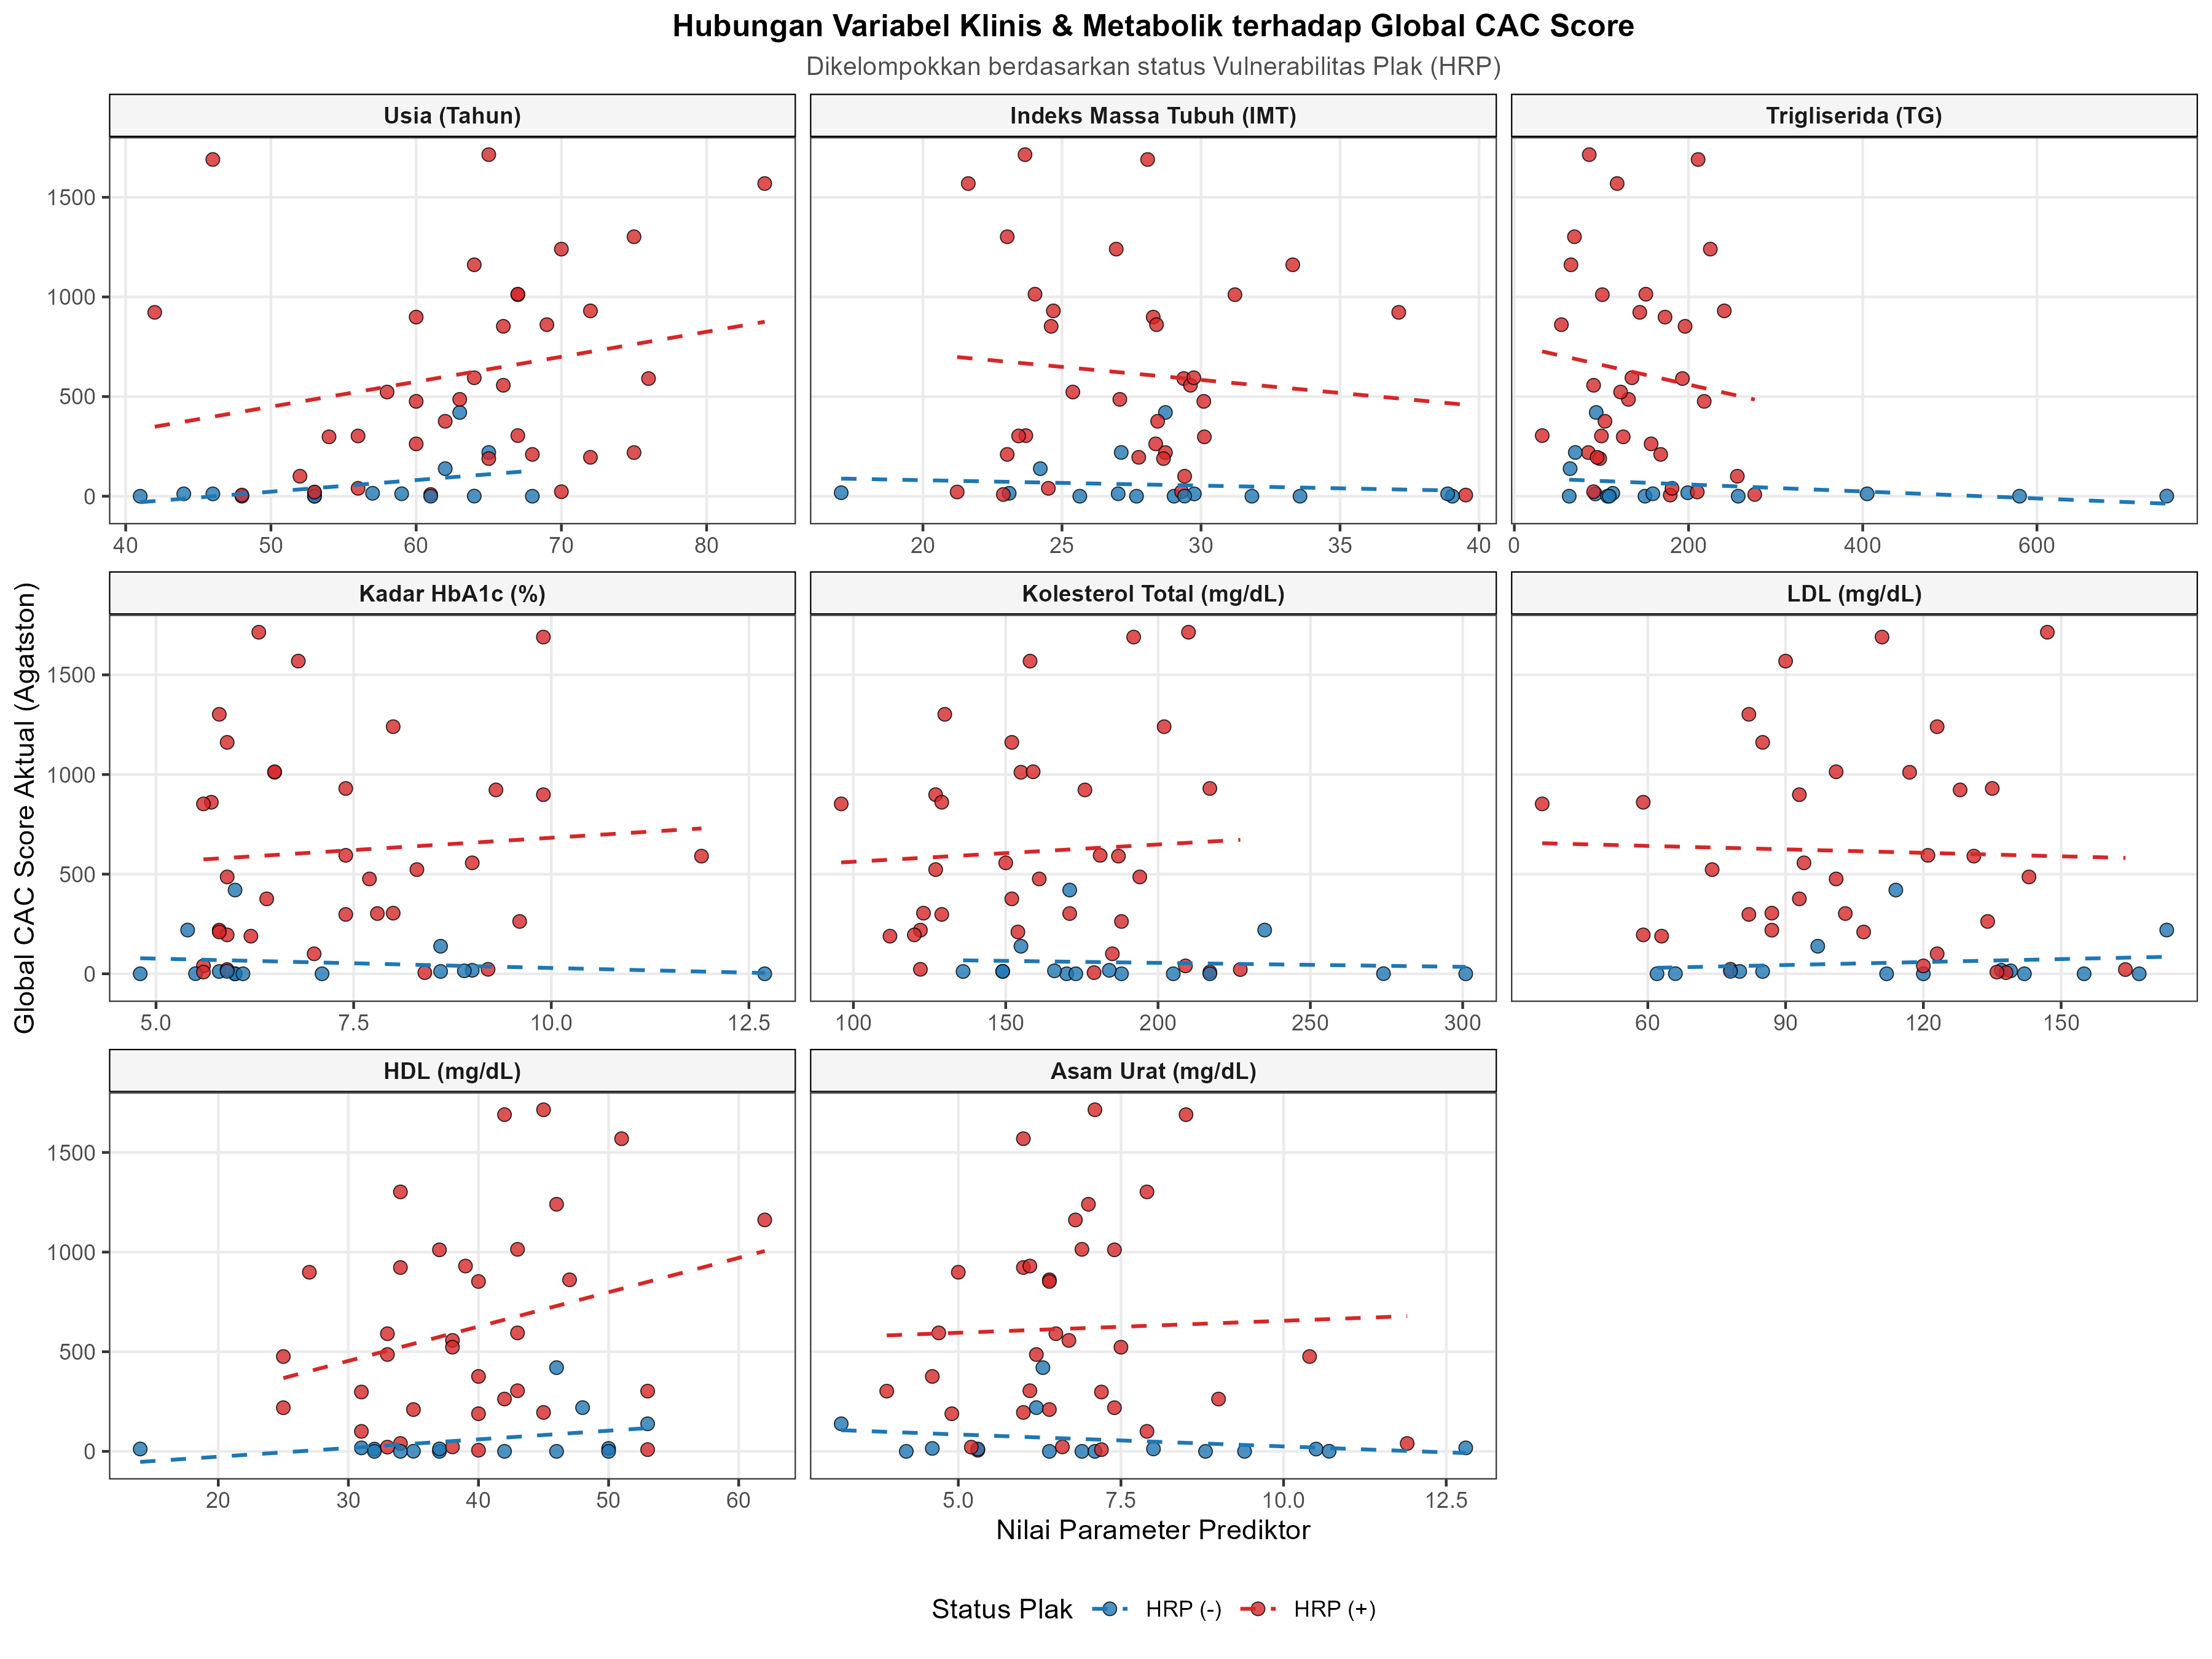
\includegraphics[keepaspectratio]{Multi_Panel_Korelasi_CAC.png}}

}

\caption{Gambar 1. Hubungan Variabel Klinis dan Metabolik terhadap
Global CAC Score Berdasarkan Status HRP}

\end{figure}%

\textbf{Analisis Multivariat Prediktor \emph{High-Risk Plaque} (HRP)}

Pemodelan regresi logistik multivariat (Generalized Linear Model)
dilakukan untuk mengevaluasi kekuatan prediktif klinis komprehensif
dengan memasukkan variabel Usia, IMT, TyHbA1c Index, dan Status CKD
(Tabel~\ref{tbl-regresi}). Hasil analisis mengonfirmasi bahwa Usia
merupakan prediktor independen yang bermakna secara statistik terhadap
pembentukan plak risiko tinggi (Odds Ratio {[}OR{]} = 1.08; 95\% CI: 1
-- 1.18; \(p\) = 0.05). Secara klinis, komplikasi fungsi ginjal
memberikan dampak risiko yang masif; pasien dengan status CKD
menunjukkan tren peningkatan probabilitas kerentanan plak hingga 2.24
kali lipat lebih tinggi dibandingkan pasien dengan ginjal normal (OR =
2.24; 95\% CI: 0.43 -- 17.16; \(p\) = 0.368). Sementara itu, variabel
TyHbA1c Index dan IMT tidak menunjukkan kemaknaan statistik parsial
secara independen dalam kohort terbatas ini.

\begin{table}

\caption{\label{tbl-regresi}\textbf{Analisis Multivariat Prediktor
High-Risk Plaque (HRP)}}

\centering{

\fontsize{12.0pt}{14.0pt}\selectfont
\begin{tabular*}{\linewidth}{@{\extracolsep{\fill}}lcccc}
\toprule
\textbf{Variabel} & \textbf{OR}\textsuperscript{\textit{1}} & \textbf{IK 95\%}\textsuperscript{\textit{2}} & \textbf{95\% CI} & \textbf{Nilai \emph{p}} \\ 
\midrule\addlinespace[2.5pt]
Usia (Tahun) & 1.08 & 1.00,  1.18 & 1.00, 1.18 & {\bfseries 0.050} \\ 
Indeks Massa Tubuh (IMT) & 1.01 & 0.87,  1.16 & 0.87, 1.16 & >0.9 \\ 
Indeks TyHbA1C & 1.05 & 0.34,  3.35 & 0.34, 3.35 & >0.9 \\ 
PGK Stadium ≥ 3 & 2.24 & 0.43,  17.2 & 0.43, 17.2 & 0.4 \\ 
\bottomrule
\end{tabular*}
\begin{minipage}{\linewidth}
\vspace{.05em}
\textsuperscript{\textit{1}}OR = Odds Ratio\\
\textsuperscript{\textit{2}}IK = Interval Kepercayaan\\
Abbreviations: CI = Confidence Interval, OR = Odds Ratio\\
\end{minipage}

}

\end{table}%

\textbf{Performa Model Prediksi dan Nomogram Klinis}

Meskipun secara parsial beberapa variabel tidak mencapai signifikansi
statistik, kombinasi holistik dari keempat parameter klinis tersebut
(Usia + IMT + TyHbA1c Index + CKD) menghasilkan daya diskriminasi
diagnostik yang solid. Analisis \emph{Receiver Operating Characteristic}
(ROC) membuktikan bahwa model multivariat ini mampu membedakan
probabilitas keberadaan HRP dengan nilai \emph{Area Under the Curve}
(AUC) sebesar 0.724 (Gambar~\ref{fig-roc}).

\begin{figure}

\centering{

\pandocbounded{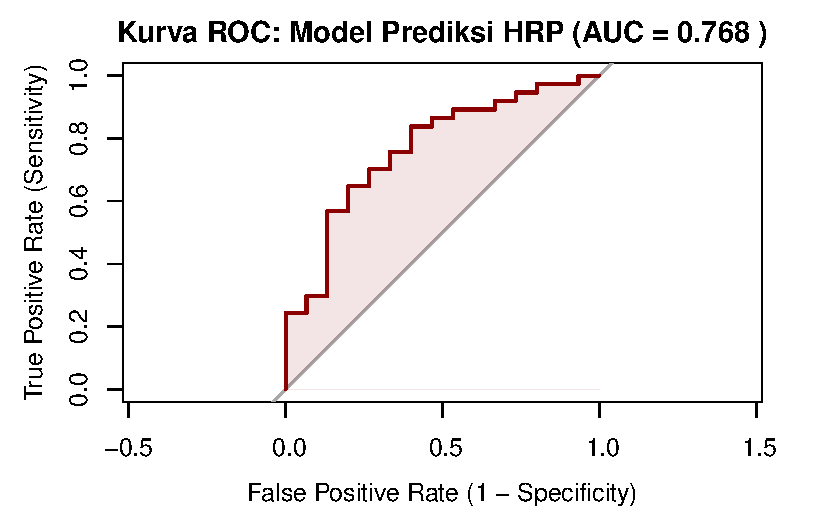
\includegraphics[keepaspectratio]{index_files/figure-pdf/fig-roc-1.pdf}}

}

\caption{\label{fig-roc}\textbf{Kinerja Diskriminatif Model Prediksi
\emph{High-Risk Plaque}.} Kurva ROC dari model komprehensif
mengintegrasikan Usia, IMT, TyHbA1c Index, dan Status Penyakit Ginjal
Kronis (CKD) dengan nilai \emph{Area Under the Curve} (AUC) sebesar
0,724.}

\end{figure}%

Model ini kemudian ditransformasikan secara visual ke dalam bentuk
nomogram klinis komprehensif guna memfasilitasi estimasi probabilitas
kemunculan \emph{vulnerable plaque} (0 - 100\%).

\begin{figure}

\centering{

\pandocbounded{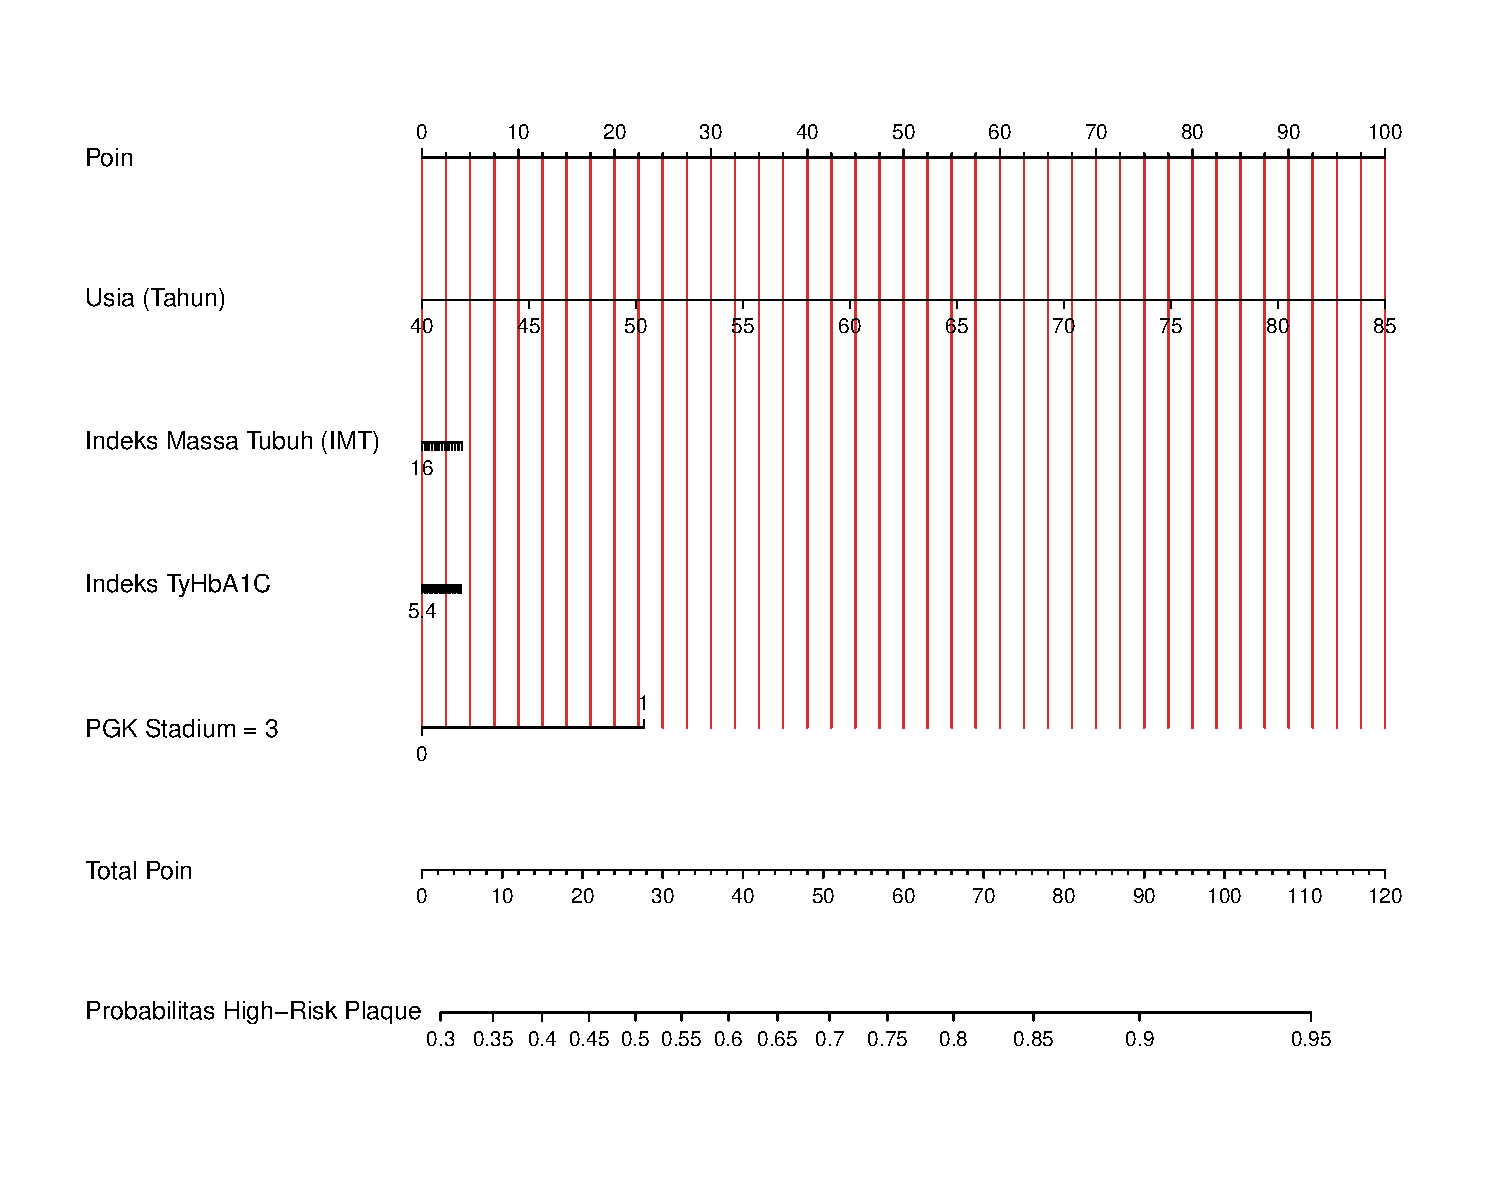
\includegraphics[keepaspectratio]{index_files/figure-pdf/fig-nomogram-1.pdf}}

}

\caption{\label{fig-nomogram}\textbf{Nomogram Klinis Komprehensif untuk
Prediksi Probabilitas \emph{High-Risk Plaque} (HRP).} Probabilitas
individual pasien diproyeksikan dengan menjumlahkan total poin (0-100)
dari keempat variabel patofisiologis: Usia, IMT, Indeks TyHbA1c, dan
Status CKD.}

\end{figure}%

Guna mengakomodasi optimalisasi translasi klinis yang lebih efisien dan
parsimonious (hanya menggunakan variabel yang terbukti independen secara
statistik), sebuah Nomogram Tereduksi juga dikembangkan dengan membuang
parameter metabolik.

\begin{figure}

\centering{

\pandocbounded{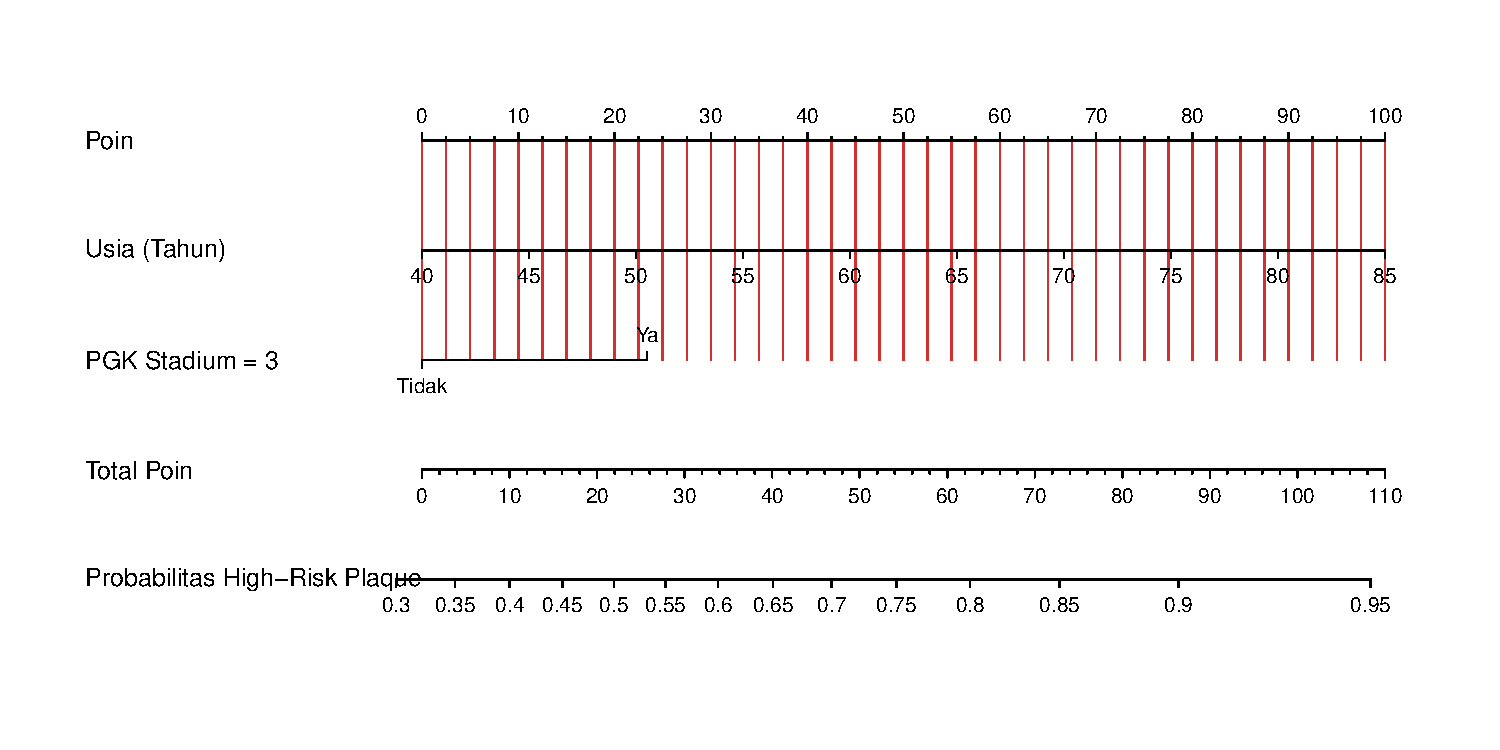
\includegraphics[keepaspectratio]{index_files/figure-pdf/fig-nomogram-reduksi-1.pdf}}

}

\caption{\label{fig-nomogram-reduksi}\textbf{Nomogram Klinis Tereduksi
(Model Sederhana).} Alat stratifikasi risiko \emph{High-Risk Plaque}
(HRP) yang dioptimalkan dengan hanya mengandalkan dua prediktor utama:
Usia dan Penyakit Ginjal Kronis (PGK) Stadium ≥ 3.}

\end{figure}%

\textbf{Analisis Prediktor Kuantitas Kalsifikasi (Global CAC Score}
\(\ge\) 100)

Selain menilai kualitas dan kerentanan plak, pemodelan sekunder
dilakukan untuk memprediksi kuantitas beban kalsifikasi secara anatomis.
Dari keseluruhan sampel, sebanyak 35 pasien (67.3\%) teridentifikasi
memiliki skor CAC \(\ge\) 100 Agatston. Berbeda dengan model prediksi
HRP komprehensif, regresi logistik untuk CAC \(\ge\) 100
(@tbl-regresi-cac) dikonstruksi secara lebih \emph{streamline} dengan
mengeksklusi Indeks Massa Tubuh (IMT) akibat kontribusi parsialnya yang
sangat minimal. Hasilnya menegaskan bahwa \textbf{Usia} menjadi
prediktor independen yang sangat kuat dan bermakna secara statistik (OR
= 1.1; 95\% CI: 1.02 -- 1.2; \(p\) = 0.021) terhadap akumulasi kalsium
anatomis.

\begin{table}

\caption{\label{tbl-regresi-cac}\textbf{Analisis Multivariat Prediktor
Kalsifikasi Koroner Moderat-Berat (CAC ≥ 100 Agatston)}}

\centering{

\fontsize{12.0pt}{14.0pt}\selectfont
\begin{tabular*}{\linewidth}{@{\extracolsep{\fill}}lcccc}
\toprule
\textbf{Variabel} & \textbf{OR}\textsuperscript{\textit{1}} & \textbf{IK 95\%}\textsuperscript{\textit{2}} & \textbf{95\% CI} & \textbf{Nilai \emph{p}} \\ 
\midrule\addlinespace[2.5pt]
Usia (Tahun) & 1.10 & 1.02,  1.20 & 1.02, 1.20 & {\bfseries 0.021} \\ 
Indeks TyHbA1C & 0.47 & 0.14,  1.40 & 0.14, 1.40 & 0.2 \\ 
PGK Stadium ≥ 3 & 1.40 & 0.28,  8.08 & 0.28, 8.08 & 0.7 \\ 
\bottomrule
\end{tabular*}
\begin{minipage}{\linewidth}
\vspace{.05em}
\textsuperscript{\textit{1}}OR = Odds Ratio\\
\textsuperscript{\textit{2}}IK = Interval Kepercayaan\\
Abbreviations: CI = Confidence Interval, OR = Odds Ratio\\
\end{minipage}

}

\end{table}%

Mempertimbangkan kontribusi Indeks Massa Tubuh (IMT) yang sangat minimal
terhadap akumulasi kalsium anatomis, variabel tersebut dieksklusi dari
model sekunder ini guna menciptakan instrumen prediksi yang lebih
\emph{streamline} dan efisien. Menariknya, meskipun dirampingkan,
integrasi ketiga variabel utama (Usia + TyHbA1c + PGK) mampu
menghasilkan diskriminasi diagnostik yang sangat baik untuk memprediksi
CAC \(\ge\) 100. Analisis ROC menunjukkan performa yang superior dengan
nilai \emph{Area Under the Curve} (AUC) mencapai \textbf{r
auc\_val\_cac} (78.2\%), seperti yang ditampilkan pada
Gambar~\ref{fig-roc-cac}.

\begin{figure}

\centering{

\pandocbounded{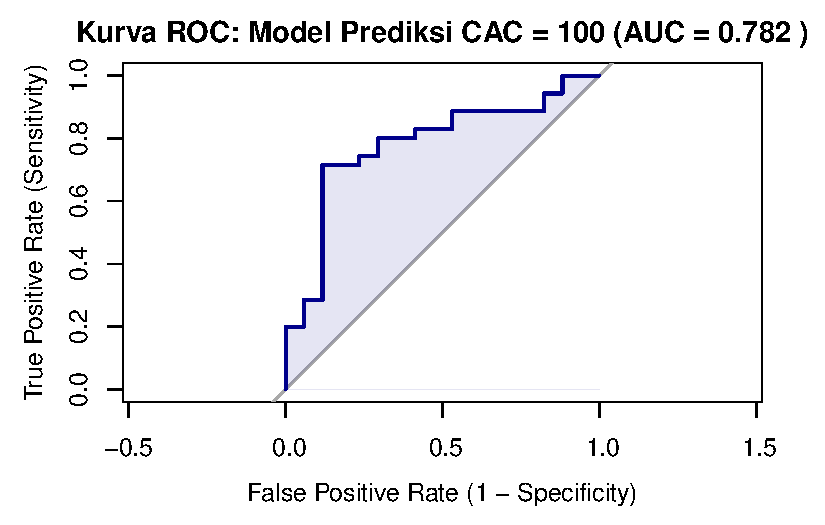
\includegraphics[keepaspectratio]{index_files/figure-pdf/fig-roc-cac-1.pdf}}

}

\caption{\label{fig-roc-cac}\textbf{Kinerja Diskriminatif Model Prediksi
Beban Kalsifikasi (CAC ≥ 100).} Kurva ROC ini menunjukkan akurasi
diagnostik yang sangat baik dengan nilai \emph{Area Under the Curve}
(AUC) sebesar 0,782.}

\end{figure}%

Berdasarkan performa tersebut, sebuah Nomogram sekunder
(Gambar~\ref{fig-nomogram-cac}) dikembangkan. Penggabungan nomogram HRP
dan nomogram CAC ini menghadirkan instrumen ``Stratifikasi Ganda'', yang
memungkinkan klinisi memprediksi dua domain vital sekaligus.

\begin{figure}

\centering{

\pandocbounded{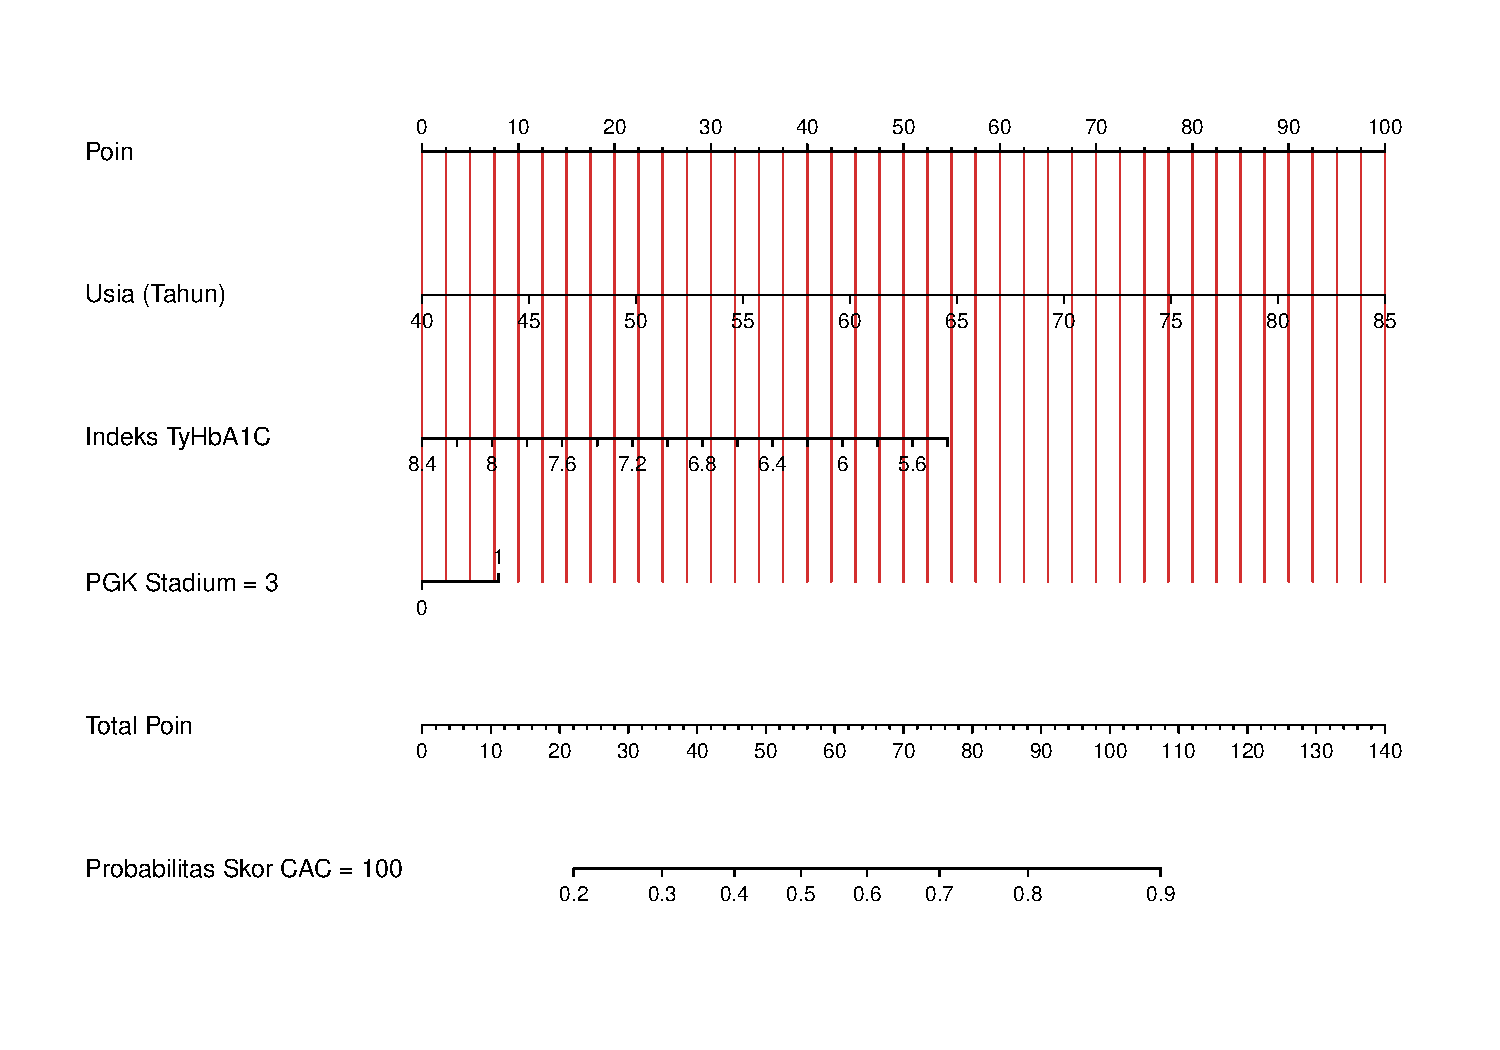
\includegraphics[keepaspectratio]{index_files/figure-pdf/fig-nomogram-cac-1.pdf}}

}

\caption{\label{fig-nomogram-cac}\textbf{Nomogram Klinis untuk Prediksi
Probabilitas Skor CAC ≥ 100 Agatston.} Instrumen ini telah dioptimalkan
(\emph{streamlined}) untuk mendampingi nomogram HRP dalam menilai risiko
beban kalsifikasi secara efisien.}

\end{figure}%

\section{Pembahasan}\label{pembahasan}

Penelitian ini mengevaluasi nilai prediktif kombinasi parameter klinis
dan kardiometabolik (Usia, IMT, Indeks TyHbA1c, dan status PGK Stadium
\(\ge\) 3) terhadap keparahan penyakit arteri koroner pada 52 pasien
diabetes serta prediabetes yang menjalani pemeriksaan CTCA. Temuan utama
studi ini mengonfirmasi bahwa pemodelan regresi logistik multivariat
yang mengintegrasikan parameter tersebut memiliki diskriminasi yang baik
dalam memprediksi \emph{High-Risk Plaque} (HRP) dengan AUC 0.724, serta
memprediksi kalsifikasi moderat-berat (CAC \(\ge\) 100) dengan AUC
0.782.

\textbf{Glukolipotoksisitas Kronis, Aktivasi Makrofag, dan Kerentanan
Plak (\emph{Plaque Vulnerability})}

Keunggulan prediktif terhadap keberadaan HRP memberikan wawasan
patofisiologis yang krusial. HRP---yang bermanifestasi sebagai
\emph{positive remodeling}, kalsifikasi bercak, dan
\emph{low-attenuation plaque}---merupakan prekursor struktural yang
sangat rentan mengalami ruptur dan memicu sindrom koroner akut. Dalam
studi ini, Indeks TyHbA1c diajukan sebagai penanda \emph{novel} yang
merepresentasikan interaksi ganda antara dislipidemia aterogenik
(hipertrigliseridemia) dan paparan hiperglikemia kronis (HbA1c). Kondisi
glukolipotoksisitas persisten memicu akumulasi AGEs dan \emph{Reactive
Oxygen Species} (ROS) yang merusak integritas endotel, memfasilitasi
infiltrasi makrofag besar-besaran yang bertransformasi menjadi sel busa
(\emph{foam cells}) di ruang subendotel.

Berdasarkan patobiologi vaskular, makrofag intratunika yang teraktivasi
ini mensekresi \emph{Matrix Metalloproteinases} secara masif yang
mendegradasi matriks ekstraseluler pada tunika media. Degradasi matriks
ke arah luar dinding epikardial inilah yang mendasari fenomena
\emph{positive remodeling} (Fenomena Glagov) sebagai upaya kompensatorik
tubuh mempertahankan ukuran lumen. Meskipun secara hemodinamik aliran
darah awal tampak tidak terganggu, remodeling ini memfasilitasi
pembentukan plak dengan inti nekrotik lipid masif dan selubung fibrosa
tipis.

\textbf{Rasionalisasi Nomogram Tereduksi}

Meskipun model multivariat komprehensif mengonfirmasi integrasi teoretis
keempat parameter utama, ukuran sampel yang terbatas pada studi ini
mengakibatkan beberapa variabel spesifik (IMT dan Indeks TyHbA1c) belum
mencapai signifikansi statistik parsial terhadap kerentanan plak.
Sebagai bentuk optimalisasi translasi klinis, studi ini juga menyajikan
Nomogram Tereduksi yang hanya mengandalkan prediktor independen terkuat
secara statistik (Usia dan status PGK). Model sederhana ini menawarkan
alternatif stratifikasi risiko yang jauh lebih cepat dan efisien di
ruang praktik IGD atau Poliklinik sibuk, tanpa mengesampingkan nilai
patofisiologis jangka panjang dari model komprehensif TyHbA1c.

\textbf{Pendekatan Stratifikasi Ganda: Kualitas Plak vs Kuantitas
Kalsifikasi}

Pengembangan dua domain nomogram (HRP dan CAC) menyoroti perbedaan
patofisiologi mendasar antara kualitas dan kuantitas aterosklerosis.
Model prediksi HRP difokuskan untuk menilai ``kualitas'' dan kerentanan
plak terhadap ruptur, yang dihipotesiskan sangat dipengaruhi oleh
fluktuasi metabolik kronis (disimbolkan oleh tren TyHbA1c). Sebaliknya,
pemodelan sekunder memvalidasi bahwa ``kuantitas'' pembentukan kalsium
yang masif (CAC \(\ge\) 100 Agatston) sebagian besar disetir secara
absolut oleh efek kumulatif degeneratif, di mana variabel Usia menjadi
prediktor tunggal yang paling mendominasi (\(p=0.021\)). Melalui
pendekatan stratifikasi ganda ini, klinisi dapat memilah pasien menjadi
fenotipe spesifik---misalnya, pasien usia muda dengan skor CAC rendah
namun probabilitas HRP tinggi (membutuhkan stabilisasi plak
anti-inflamasi), berbanding pasien geriatri dengan probabilitas CAC
masif (membutuhkan intervensi agresif akibat obstruksi kronis).

\textbf{Peran Dominan Usia dan Poros Kardiorenal}

Dalam seluruh pemodelan, usia muncul sebagai penentu utama. Proses
aterosklerosis pada dasarnya adalah patologi kumulatif yang bergantung
pada waktu (\emph{time-dependent}), di mana durasi paparan terhadap sel
endotel memperbesar probabilitas degenerasi. Selain faktor usia,
kehadiran Penyakit Ginjal Kronis (PGK Stadium \(\ge\) 3) terbukti
memberikan tren peningkatan risiko kerentanan plak yang masif. Nefropati
diabetik bertindak sebagai katalisator melalui poros kardiorenal
(\emph{cardiorenal syndrome}). Retensi toksin uremik dan gangguan
metabolisme mineral pada pasien PGK berinteraksi sinergis memicu
degradasi stabilitas koroner secara progresif.

\textbf{Keterbatasan Penelitian}

Studi ini memiliki beberapa keterbatasan yang perlu dicatat. Desain
potong lintang (\emph{cross-sectional}) membatasi kemampuan studi untuk
menyimpulkan hubungan kausalitas sejati secara longitudinal. Selain itu,
ukuran sampel pada kohort \emph{single-center} ini (N=52) membatasi
kekuatan statistik parsial (seperti terlihat pada variabel IMT dan
TyHbA1c), dan masih memerlukan ekspansi lebih lanjut guna memperkuat
\emph{confidence interval}. Penelitian lanjutan dengan validasi kohort
eksternal multisentris sangat disarankan guna mengonfirmasi keandalan
serta kalibrasi dari instrumen stratifikasi ganda yang dihasilkan.

\section{Simpulan}\label{simpulan}

Kombinasi parameter klinis dan kardiometabolik yang mencakup Usia,
Indeks Massa Tubuh (IMT), Indeks TyHbA1c, dan status Penyakit Ginjal
Kronis (PGK Stadium \(\ge\) 3) terbukti memiliki kemampuan diskriminasi
diagnostik yang solid. Studi ini memperkenalkan inovasi pendekatan
``Stratifikasi Ganda'' melalui pengembangan tiga nomogram klinis
aplikatif. Nomogram pertama (komprehensif dan tereduksi) dirancang
secara spesifik memprediksi kerentanan kualitas plak (\emph{High-Risk
Plaque} / HRP) dengan AUC 0.724. Sementara itu, nomogram sekunder
memprediksi kuantitas beban kalsifikasi moderat-berat (CAC \(\ge\) 100)
dengan akurasi tinggi (AUC 0.782) yang sangat didominasi oleh faktor
degeneratif usia. Penggunaan instrumen ganda ini memungkinkan para
klinisi melakukan stratifikasi risiko kardiovaskular secara holistik dan
non-invasif, guna menyeleksi prioritas rujukan pemeriksaan
\emph{Computed Tomography Coronary Angiography} (CTCA) dan personalisasi
terapi secara presisi.

\section{Daftar Pustaka}\label{daftar-pustaka}




\end{document}
